\documentclass[a4paper,12pt]{article} 
\usepackage{baseset}
\DeclareSymbolFont{operators}{OT1}{ntxtlf}{m}{n}
\SetSymbolFont{operators}{bold}{OT1}{ntxtlf}{b}{n}
\usepackage{wasysym}
\usepackage{multirow}
\graphicspath{{images/}}
\DeclareGraphicsExtensions{.pdf,.png,.jpg}

%Заговолок
\author{Красоткина Виктория}

\title{Лабораторная работа 1.2.4

Определение главных моментов инерции твердых тел с помощью крутильных колебаний}

\date{28 ноября 2022 г.}

\begin{document}

\maketitle
\thispagestyle{empty}

\newpage
\setcounter{page}{1}

\textbf{Цель:}
Измерить периоды крутильных колебаний рамки при различных положениях закрепленного
в ней тела, проверить теоретическую зависимость между периодами крутильных колебаний тела
относительно различных осей, определить моменты инерции относительно нескольких осей для каждого тела, 
по ним найти главные моменты инерции тела и посторить эллипсоид инерции.\\

\textbf{Приборы:}
\begin{itemize}
    \item установка для получения крутильных колебаний
    \item набор исследуемых твердых тел
    \item секундомер
\end{itemize}

\subsection*{Теоретическая часть}
Инерционные свойства твердого тела при вращении определяется
 пространственным распределением. Оно характеризуется тензором инерции тела. Тензор инерции твердога тела
 является симметричным тензором 2-ого ранга $J\in  T_{2}^{0}(V)$ и имеет 6 независимых компонент,
 которые в прямоугольной декартовой системе координат выражаются как:
\begin{equation}
    J_{ij}=\int (\delta _{ij}r^{2}-r_{i}r_{j}) \ dm =J_{ji}, \ \ \ J = J_{ij} \cdot h^{i} \otimes h^{j}
\end{equation}
 где $r$ — расстояния от точек до центра, относительно которого вычисляется тензор инерции,
а $r_{i}$ — координатные компоненты соответствующих отрезков, $i$ и $j$ — номера координат (от 1 до 3).\\
Если для какой либо системы координат все 6 компонент известны, то момент инерции тела относительно
 произвольной оси $l$, проходящей через начало координат может быть вычислен по формуле:
\begin{equation}
    J_{l}=n^{j}n^{i}J_{ij}=\overrightarrow{n}^{T} J \overrightarrow{n} 
\end{equation}
где $\overrightarrow{n}$ - единичный вектор-столбец который задает направление оси, $J$ - тензор инерции.\\
А момент импульса $\vec  {L}$ и вращательная энергия тела $E_{\text{вращ}}$ тогда будут выражаться как:
\begin{equation}
    E_{\text{вращ}}={1 \over 2}\ {\vec {\omega }}^{\,T}\cdot J\cdot {\vec {\omega }} ={1 \over 2}\sum _{{ij}}\omega^{i}J_{{ij}}\omega^{j}
\end{equation}
\begin{equation}
    {\vec  {L}}=J \cdot {\vec  {\omega }}, \ \ \ \ L_{i}=\sum _{j}J_{{ij}}\omega^{j}
\end{equation}
Отложим вдоль оси $l$ из начала координат радиус-вектор $r$
равный по длине $1/\sqrt{J_{l}}$. Проведем множество таких отрезков, соответствующих различным направлениям оси $l$.
 Геометрическое место концов указанных отрезков, является поверхность второго порядка - эллипсоид. Этот эллипсоид принято называть
 эллипсоидом инерции. Он жестко связан с телом для которого он постоен. Знание эллипсоида инерции позволяет найти момент инерции тела
относительно любой оси, проходящей через центр эллипсоида. Длина отрезка $r$ будет определять момент инерции тела относительно оси $l$:
\begin{equation}
    J_{l} = \frac{1}{r^2}
    \label{ссылка}
\end{equation}
Как и всякий симметричный тензор второго ранга может быть диагонализован некоторой заменой координат. 
Пусть система координат, в которой он диагонализован имеет оси $Ox,Oy,Oz$, тогда эти оси совпадают с главными осями тела.
Полученные диагональные элементы $J_{x}, J_{y}, J_{z}$ называются главными моментами инерции тела, а ур-ие эллипсоида
 инерции в этих координатах примит вид:
\begin{equation}
    1 = J_{x}r^{2}_{x}+J_{y}r^{2}_{y}+J_{z}r^{2}_{z}
\end{equation}
Крутильные колебания рамки с телом описываются уравнением:
\begin{equation}
    (I+I_{p})\frac{d^2 \phi}{d t^2} = -f \cdot \phi
\end{equation}
Здесь $I$ и $I_{p}$ - моменты инерции тела и рамки относительно
 оси вращения, $\varphi$ - угол поворота рамки, меняющийся со
временем $t$, $f$ - модуль кручения проволоки. Период крутильных
 колебаний рамки с телом определяется формулой:
\begin{equation}
    T = 2\pi\sqrt{\frac{I+I_{p}}{f}}
\end{equation}
На рисунке показано, как проходят оси вращения в параллелепипеде.
 Оси АА', BВ' и СС' являются главными. Моменты инерции относительно
этих осией обозначим соотственно $J_{x}, J_{y}, J_{z}$.\\

 \begin{figure}[!h]
    \begin{center}
        \includegraphics[scale=1]{kyb}
        \caption{Оси вращения прямоугольного параллелепипеда}
        \label{graphic1}
    \end{center}
\end{figure}

Момент инерции $I_{D}$ при вращении относительно диагонали DD' выражается
 через главные моменты с помощью формулы:
\begin{equation}
    I_{d}=I_{x}\frac{a^2}{d^2}+I_{y}\frac{b^2}{d^2}+I_{z}\frac{c^2}{d^2}
\end{equation}
Используя связь момента инерции с периодом крутильных колебаний
получаем соотношение между периодами колебаний относительно осей DD', ЕE',
ММ' и PР' с периодами крутильных колебаний относительно главных осей.
$$(a^2+b^2+c^2)T^2_{D}=a^2 T^2_{x}+b^2 T^2_{y}+c^2 T^2_{z}$$
$$(b^2+c^2)T^2_{E}=b^2 T^2_{y}+c^2 T^2_{z}$$
$$(a^2+c^2)T^2_{P}=a^2 T^2_{x}+c^2 T^2_{z}$$
$$(a^2+b^2)T^2_{M}=a^2 T^2_{x}+b^2 T^2_{y}$$
Эти соотношения также необходимо проверить экспериментально.

\subsubsection*{Экспериментальная установка}

\begin{figure}[!h]
    \begin{center}
        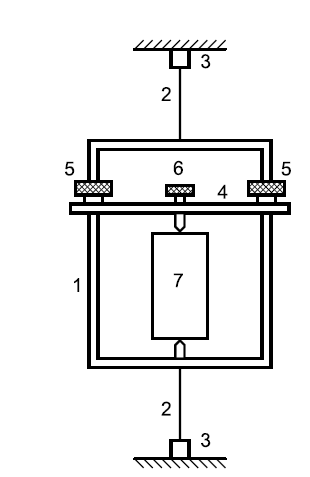
\includegraphics[scale=1]{ystanovka}
        \caption{Схема установки}
        \label{graphic1}
    \end{center}
\end{figure}

В данной работе используется устройство для получения крутил-
ных колебаний, изображенное на риcунке. Рамка 1 жестко соединена
с проволокой 2, закрепленной вертикально в специальных зажимах
3, позволяющих сообщить начальное закручивание для возбуждения
крутильных колебаний вокруг вертикальной оси. В рамке с помощью
планки 4, гаек 5 и винта 6 закрепляется твердое тело 7. На теле име-
ются специальные выемки, позволяющие его закрепить так, чтобы ось
вращения проходила в теле под различными углами через центр масс.

\end{document}

\section{Результаты эксперимента и обраюотка данных}
\begin{itemize}
    \item Для начала установим геометрические параметры исследуемых тел. 
Штангенциркулем измеряем размеры и заносим в табличку.
\begin{table}[!h]
    \centering
    \begin{tabular}{|l|l|l|l|} \hline
        - & m, гр & d, см & h, см  \\ \hline
        Мелкий цилиндр & 1569 & 12.45 & 1.68  \\ \hline
        Средний цилиндр & 2264 & 88.3 & 49  \\ \hline
    \end{tabular}
    \caption{Измерения для цилиндров}
\end{table}

\begin{table}[!ht]
    \centering
    \begin{tabular}{|l|l|l|}
    \hline
        m, гр & a, см  \\ \hline
        1084 & 92.7  \\ \hline
    \end{tabular}
    \caption{Измерения для куба}
\end{table}

\begin{table}[!ht]
    \centering
    \begin{tabular}{|l|l|l|l|l|}
    \hline
        m, гр & c, см & b, см & a, см  \\ \hline
        2082 & 150.3 & 50.5 & 100.2  \\ \hline
    \end{tabular}
    \caption{Измерения для прямоугольника}
\end{table}
Теперь по этим данным вычислим главные моменты инерции и их погрешность:
$$\varepsilon \approx \sqrt{\varepsilon^2_{a}+\varepsilon^2_{a}}\approx 0.1 \% $$
\begin{description}
    \item[Маленький цилиндр]Моменты инерции относительно главных осей:
     $I_{z}$-относительно вертикальной оси, $I_{x}$-относительно горизонтальной оси.
$$I_{z}= 3.04 \pm 0.01 \ \text{гр}\cdot \text{м}^2, \ \ \ I_{x}= 3.08 \pm 0.01 \ \text{гр}\cdot \text{м}^2$$
    \item[Средний цилиндр]
$$I_{z}= 2.21 \pm 0.01 \ \text{гр}\cdot \text{м}^2, \ \ \ I_{x}= 2.66 \pm 0.01 \ \text{гр}\cdot \text{м}^2$$
    \item[Куб]Для куба момент инерции относительно любой оси равны.
$$I_{z}= 9.32 \pm 0.01 \ \text{гр}\cdot \text{м}^2$$
    \item[Параллелепипед]Моменты инерции относительно главных осей:
    $I_{z}$-относительно вертикальной оси CC', $I_{x}$-относительно горизонтальной оси AA',
    $I_{y}$-относительно горизонтальной оси BB'
$$I_{z}= 13.11 \pm 0.01 \ \text{гр}\cdot \text{м}^2, \ \ \ I_{x}= 26.17 \pm 0.02 \ \text{гр}\cdot
 \text{м}^2, \ \ \ I_{y}= 33.97 \pm 0.02 \ \text{гр}\cdot \text{м}^2$$
\end{description}

    \item Далее определим периоды колебаний для пустой рамки, и всех остальных тел при различном положении
относительно оси колебаний. Отсчитваем 10-15 колебаний, проводя каждое измерение 3 раза.
Также перед каждой серией измерений убеждаемся в правильности выборе амплитуды: амплитуда выбрана правильно, если при уменьшении ее
в два раза период колебаний, определяемый по 10-15 колебаниям, остается тем же. Заносим данные для разных фигур в табличку.
Погрешность измерения времени обусловлена ошибкой округления и равна: $\varepsilon_{T} \approx 0.5 \% $ при 10 измерениях и
$\varepsilon_{T} \approx 0.3 \% $ при 15 измерениях.
\begin{description}
    \item[Рамка]Измерения для рамки: 
    \begin{table}[!ht]
        \centering
        \begin{tabular}{|l|l|l|l|l|l|} \hline
            Рамка & $N$ & $t_{N1}$,с & $t_{N2}$,с & $t_{N3}$,c & $T$,c \\ \hline
            $T_{OZ}$ & 10 & 44.4 & 44.3 & 44.4 & 4.44  \\ \hline
        \end{tabular}
    \end{table}
    \item[Цилиндры]Измерения для цилиндров:
    \begin{table}[!ht]
        \centering
        \begin{tabular}{|l|l|l|l|l|l|l|}
        \hline
            Цилиндр маленький & $N$ & $t_{N1}$,с & $t_{N2}$,с & $t_{N3}$,c & $T$,c & $1/\sqrt{T^2-T^2_{p}}, 10^{-2} c^{-1}$  \\ \hline
            $T_{OZ}$ & 15 & 90.2 & 90.7 & 90.1 & 6.02 & 24.58  \\ \hline
            $T_{OX}$ & 15 & 79.1 & 79.3 & 79 & 5.28 & 35.10  \\ \hline
            Цилиндр средний & $N$ & $t_{N1}$,с & $t_{N2}$,с & $t_{N3}$,c & $T$,c & $1/\sqrt{T^2-T^2_{p}}, 10^{-2} c^{-1}$  \\ \hline
            $T_{OZ}$ & 10 & 55.8 & 55.7 & 55.9 & 5.58 & 29.59  \\ \hline
            $T_{OX}$ & 10 & 52.6 & 52.4 & 52.4 & 5.25 & 35.77  \\ \hline
        \end{tabular}
    \end{table}
    \item[Куб]Измерения для куба:
    \begin{table}[!ht]
        \centering
        \begin{tabular}{|l|l|l|l|l|l|l|}
        \hline
            куб & $N$ & $t_{N1}$,с & $t_{N2}$,с & $t_{N3}$,c & $T$,c & $1/\sqrt{T^2-T^2_{p}}, 10^{-2} c^{-1}$  \\ \hline
            $T_{EE'}$ & 15 & 79.2 & 78.8 & 79.5 & 5.28 & 35.05  \\ \hline
            $T_{DD'}$ & 15 & 78.8 & 79 & 79 & 5.26 & 35.41  \\ \hline
            $T_{OZ(CC')}$ & 10 & 53 & 52.8 & 52.7 & 5.28 & 34.92  \\ \hline
        \end{tabular}
    \end{table}
    \item[Параллелепипед]Измерения для параллелепипеда:
    \begin{table}[!ht]
        \centering
        \begin{tabular}{|l|l|l|l|l|l|l|}
        \hline
            Параллелепипед & $N$ & $t_{N1}$,с & $t_{N2}$,с & $t_{N3}$,c & $T$,c & $1/\sqrt{T^2-T^2_{p}}, 10^{-2} c^{-1}$  \\ \hline
            $T_{OZ(CC')}$ & 10 & 55.7 & 55.6 & 55.4 & 5.56 & 29.93  \\ \hline
            $T_{OX(AA')}$ & 10 & 65.6 & 64.9 & 65.1 & 6.52 & 20.94  \\ \hline
            $T_{OY(BB')}$ & 10 & 69.9 & 69.9 & 69.7 & 6.98 & 18.55  \\ \hline
            $T_{DD'}$ & 10 & 59.3 & 59.5 & 59.5 & 5.94 & 25.31  \\ \hline
            $T_{EE'}$ & 10 & 57.3 & 56.9 & 57.1 & 5.71 & 27.85  \\ \hline
            $T_{MM'}$ & 10 & 66.1 & 66.6 & 65.9 & 6.62 & 20.37  \\ \hline
            $T_{PP'}$ & 10 & 59.2 & 58.5 & 58.9 & 5.89 & 25.87  \\ \hline
        \end{tabular}
    \end{table}
\end{description}

    \item Проверим теоретически предсказанные соотношения для связи периодов
 колебаний вокруг побочных осей $DD',EE',MM',PP'$ с периодами колебаний вокруг главных осей $OX,OY,OZ$ пользуясь формулами \dots.
 Учтем также что параметры тел были измерены намного более точнее чем период колебаний, поэтому можем счтать, что $\varepsilon_{T^2} \approx 1\%$
\begin{description}
    \item[Ось DD']теоретический результат: $T^{2}_{DD'}=35.5 \pm 0.1 \ c^2$,\\ экспериментальный результат: $T^{2}_{DD'}=35.3 \pm 0.2$
    \item[Ось EE']теоретический результат: $T^{2}_{EE'}=32.7 \pm 0.1 \ c^2$,\\ экспериментальный результат: $T^{2}_{EE'}=32.6 \pm 0.2$
    \item[Ось MM']теоретический результат: $T^{2}_{MM'}=43.8 \pm 0.1 \ c^2$,\\ экспериментальный результат: $T^{2}_{MM'}=43.8 \pm 0.2$
    \item[Ось PP']теоретический результат: $T^{2}_{PP'}=34.5 \pm 0.1 \ c^2$,\\ экспериментальный результат: $T^{2}_{PP'}=34.6 \pm 0.2$
\end{description}
Как видно, теоретические предсказания хорошо согласуются с экспериментальными в пределах погрешности, что поддтверждает предположение о том,
 что оси $OX,OY,OZ$ являются главными осями тела.\\
    \item Теперь по полученным ранее данным построим эллипсоид инерции для параллелограмма и куба. За длину радиус вектора примим
$r=100/\sqrt{T^2-T^2_{p}}$. Строить эллипсы будем методом наименьших квадратов. Т.к параметричеческое ур-ие эллипса выглядит как:\\
$y=b \cdot \sin(\varphi), x= a \cdot \cos(\varphi)$ То зависимость координаты $x,y$ от соответственно $sin(\varphi),\cos(\varphi)$ линейная и
проходит через начало координат. Тогда зная 
длину радиус вектора и углы под которыми направлены побочные оси к главным осям, проводим аппроксимацию методом наименьших квадратов
 и строим эллипс с полученными параметрами.
$$a=\frac{\langle x \cdot \cos(\varphi)\rangle }{\langle \cos(\varphi)^2 \rangle }, \ \ \ b=\frac{\langle y \cdot \sin(\varphi)\rangle }{\langle \sin(\varphi)^2 \rangle }$$
\begin{description}
    \item[Цилиндры]Мелкий цилиндр: $a = 35.1 \cdot 10^{-2}c^{-1}$ ,$b = 24.6 \cdot 10^{-2}c^{-1}$\\
Средний цилиндр: $a = 35.8  \cdot 10^{-2}c^{-1}$ ,$b = 29.6 \cdot 10^{-2}c^{-1}$
    \item[Куб] Для куба эллипсоид инерции - шар. Примим за его радиус средний по
всем сериям измерений. $r = 35.0 \cdot 10^{-2}c^{-1}$
    \item[Параллелепипед]Проводим аппроксимацию эллипсом для 3 разных сечений
 и заносим результаты в табличку.
\end{description}

\begin{table}[!ht]
    \centering
    \begin{tabular}{|l|l|l|} \hline
        Параллелограмм & a & b  \\ \hline
        $XOZ$ & 22.8 & 27.5  \\ \hline
        $YOZ$ & 20.1 & 28.6  \\ \hline
        $XOY$ & 20.6 & 19.1  \\ \hline
    \end{tabular}
\end{table}

Причем так как в двух разных сечениях одной из осью является одна и та же ось вращения с одним и тем же
 моментом инерции, то разумно принять за истинное значение полуосиоси, усредненное по этим двум аппроксимациям, а за ее погрешность, ее париацию.
Тогда для итоговых значений полуосей и их погрешностей имеем:
$c=r_{OZ(CC')}= 28.05 \pm 0.55 \cdot 10^{-2}c^{-1}$\\
$a=r_{OX(AA')}= 21.07 \pm 1.1 \cdot 10^{-2}c^{-1}$\\
$b=r_{OY(BB')}= 19.06 \pm 0.5 \cdot 10^{-2}c^{-1}$

\begin{figure}[!ht]
    \begin{center}
    \begin{minipage}[h]{0.49\linewidth}
    \includegraphics[width=1\linewidth]{small}
    \caption{Сечение эллипсоида инерции для меньшенго цилиндра} %% подпись к рисунку
    %\label{ris:experimoriginal} %% метка рисунка для ссылки на него
    \end{minipage}
    \hfill
    \begin{minipage}[h]{0.49\linewidth}
    \includegraphics[width=1\linewidth]{middle}
    \caption{Сечение эллипсоида инерции для большего цилиндра}
    %\label{ris:experimcoded}
    \end{minipage}
    \end{center}
\end{figure}

\begin{figure}[!ht]
    \begin{center}
    \begin{minipage}[h]{0.49\linewidth}
    \includegraphics[width=1\linewidth]{kyb2}
    \caption{Сечение эллипсоида инерции куба} %% подпись к рисунку
    %\label{ris:experimoriginal} %% метка рисунка для ссылки на него
    \end{minipage}
    \hfill
    \begin{minipage}[ht]{0.49\linewidth}
    \includegraphics[width=1\linewidth]{XOY}
    \caption{Сечение эллипсоида инерции параллелограмма в плоскости XOY}
    %\label{ris:experimcoded}
    \end{minipage}
    \end{center}
\end{figure}

%\begin{figure}[!ht]
%    \centering
%    \includegraphics[scale=0.5]{kyb2}
%    \caption{Сечение эллипсоида инерции куба}
%\end{figure}

\begin{figure}[!ht]
    \begin{center}
    \begin{minipage}[h]{0.49\linewidth}
    \includegraphics[width=1\linewidth]{XOZ}
    \caption{Сечение эллипсоида инерции параллелограмма в плоскости XOZ} %% подпись к рисунку
    %\label{ris:experimoriginal} %% метка рисунка для ссылки на него
    \end{minipage}
    \hfill
    \begin{minipage}[ht]{0.49\linewidth}
    \includegraphics[width=1\linewidth]{YOZ}
    \caption{Сечение эллипсоида инерции параллелограмма в плоскости YOZ}
    %\label{ris:experimcoded}
    \end{minipage}
    \end{center}
\end{figure}

%\begin{figure}[!ht]
%    \centering
%    \includegraphics[scale=0.5]{XOY}
%    \caption{Сечение эллипсоида инерции параллелограмма в плоскости XOY}
%\end{figure}

    \item Проверим насколько теоретически предсказанные моменты инерции для параллелограммма относительно
главных осей с полученным экспериментальным результатоом, пользуясь тензором инерции.
Вычислим отношения моментов инерции вдоль главных осе. Погрешность экспериментального значения оценим как:\\
$\varepsilon_{Ji/Jj}=2\sqrt{\varepsilon^2_{ri}+\varepsilon^2_{rj}} \approx 10 \%$\\
Погрешность теоретического пренебрежимо мала и порядка $1\%$.\\
Теоретичесое значение: $J_{x}/J_{z}= 2$, экспреиментальное $J_{y}/J_{z}=c^2/a^2=1.8 \pm 0.2$\\
Теоретичесое значение: $J_{y}/J_{z}= 2.6 $, экспреиментальное $J_{y}/J_{z}=c^2/b^2=2.2 \pm 0.3$\\
Теоретичесое значение: $J_{y}/J_{x}= 1.3 $, экспреиментальное $J_{y}/J_{x}=a^2/b^2=1.2 \pm 0.1$\\
\end{itemize}

\section{Выводы}

В ходе работы были измерены периоды колебаний относительно различных осей.
Была поддтверждена теоретическая зависимость между периодами крутильных колебаний тела относительно 
различных осей. По ним были установлены положения главных осей тела и вычислены моменты инерции относительно этих осей.
По этим данным был построен вид эллипсоида инерции.\\
 Также можем заметить, что точки не идеально ложатся на построенную кривую, что вероятно обсуловленно
особенностями установки(затуханием,провисанием или возникающими эффектами) и случайной погрешностью, связанной
со скоростью реакции человека. Таким образом использование нашей установки дает некоторую приличную погрешность, 
но ее точности вполне достаточно для получения интересующих нас выводов. Поэтому, так как точки хорошо ложатся на эллипс,
мы можем сделать вывод о справедливости теоретических формул.
По виду эллипсоида инерции были вычеслены соотношения между моментами инерции тела относительно главных осей,
которые совпадают с теоретическим расчетом в пределах погрешности.

\end{document}